%-----------------------------------------------------------------------------
%
%               Template for sigplanconf LaTeX Class
%
% Name:         sigplanconf-template.tex
%
% Purpose:      A template for sigplanconf.cls, which is a LaTeX 2e class
%               file for SIGPLAN conference proceedings.
%
% Author:       Paul C. Anagnostopoulos
%               Windfall Software
%               978 371-2316for the
%               paul@windfall.com
%
% Created:      15 February 2005
%
%-----------------------------------------------------------------------------


\documentclass{sigplanconf}  %[preprint]

% The following \documentclass options may be useful:
%
% 10pt          To set in 10-point type instead of 9-point.
% 11pt          To set in 11-point type instead of 9-point.
% authoryear    To obtain author/year citation style instead of numeric.

\usepackage{amsmath}
\usepackage{amssymb}
\usepackage{amsthm}

\usepackage{multicol}
\usepackage{multirow}
\usepackage{graphicx}
\usepackage{color}
\usepackage{subfigure}
\usepackage{epsfig}
\usepackage{fancybox}
\usepackage{fancyvrb}

\usepackage{amssymb}
\usepackage{amsthm}

\usepackage{hyperref} % comes last, as it redefines a couple of commands
\hypersetup{
    colorlinks,%
    citecolor=black,%
    filecolor=black,%
    linkcolor=black,%
    urlcolor=blue
}

\DefineVerbatimEnvironment{colorcode}%
        {Verbatim}{fontsize=\small,commandchars=\\\{\}}   % \normalsize
        %{Verbatim}{fontsize=\scriptsize,commandchars=\\\{\}}


\definecolor{DikuRed}{RGB}{130,50,32}
\newcommand{\emp}[1]{\textcolor{DikuRed}{ #1}}
\definecolor{CosGreen}{RGB}{10,100,70}
\newcommand{\emphh}[1]{\textcolor{CosGreen}{ #1}}


\newcommand{\mymath}[1]{$ #1 $}
\newcommand{\myindx}[1]{_{#1}}
\newcommand{\myindu}[1]{^{#1}}
\newcommand{\mymathbb}[1]{\mathbb{#1}}

\hyphenation{ho-mo-mor-phism}
\hyphenation{list-ho-mo-mor-phism}
\hyphenation{mul-ti-pli-ca-tion}
\hyphenation{re-le-vant}
\hyphenation{asso-ci-a-ti-vi-ty}


%%%%%%%%%%%%%%%%%%%%%%%
% comments
\usepackage{color}
\newcommand{\comment}[2]{\textcolor{red}{\scriptsize \textsf \textbf{#1:}{#2}}}

% to switch comments off, activate this definition
% \renewcommand{\comment}[2]{}

%%%%%%%%%%%%%%%%%%%%%%%

\begin{document}

\conferenceinfo{FHPC'13,} {September 23, 2013, Boston, Massachusets.}
\CopyrightYear{2013}
%\copyrightdata{978-1-4503-1577-7/12/09}


\title{A Structural-Analysis Algorithm for Fusion}
\subtitle{$\mathcal{L}_0$ Status Report}
%\subtitle{Subtitle Text, if any}

%%%%%%%%%%%%%%%%%%%
%%% AUTHORS INF %%%
%%%%%%%%%%%%%%%%%%%

\authorinfo{Troels Henriksen, Cosmin E. Oancea}
           {HIPERFIT, Department of Computer Science, University of Copenhagen (DIKU)}
           {cosmin.oancea@diku.dk, athas@sigkill.dk}


%%%%%%%%%%%%%%%%%%%
%%%%%%%%%%%%%%%%%%%
%%%%%%%%%%%%%%%%%%%

\maketitle
%\renewcommand{\comment}[2]{}



\begin{abstract}

Fusion is one of the most important code transformations as it 
has the potential to substantially optimize both the memory hierarchy 
time overhead and (sometimes asymptotically) the space requirement.
%
In imperative languages, the legality of loop-fusion is typically 
verified by dependency analysis on arrays applied at loop-nest level.
Such analysis, however, has often been labeled as ``heroic effort''
and, if at all, is supported only in its simplest and most
conservative form in industrial compilers.  

In functional languages, fusion is naturally and more easily derived
as a producer-consumer relation between program constructs that expose
a richer, higher-order algebra of program invariants, 
%from the richer, higher-order semantics of program invariants, 
such as the {\tt map-reduce} list homomorphisms. %algebra.   

Related implementations in the functional context typically 
apply fusion only when the to-be-fused producer is used exactly once,
i.e., in the consumer.   This guarantees that the transformation is
conservative: the resulting program does not duplicate computation.

We show that the above restriction is more conservative than needed,
and present a structural-analysis algorithm, inspired
from the {\tt T$_1$-T$_2$} transformation for reducible data flow,
that enables fusion even in some cases when the producer is used 
in different consumers {\em and} without duplicating computation.  

We report an implementation of the fusion algorithm for a 
{\em functional}-core language, named $\mathcal{L}_0$, which is intended 
to support {\em nested} parallelism across {\em regular} 
multi-dimensional arrays.  We succinctly describe $\mathcal{L}_0$'s
semantics and the compiler infrastructure on which the fusion
transformation relies.

\end{abstract}

%\category{CR-number}{subcategory}{third-level}
\category{D.1.3}{Concurrent Programming}{Parallel Programming}
%\category{D.1.3}{Programming Techniques}{Concurrent Programming}%%[Parallel Programming]
\category{D.3.4}{Processors}{Compiler}


\terms
Performance, Design, Algorithms

\keywords
fusion, autoparallelization, functional language

\section{Introduction}
\label{sec:Introduction}

%%%%%%%%%%%%%%%%%%%%%%%%%%%%%%%%%%%%%%%%%%%%%%%%%%%%%%%%%%%%%%
%%% HL Introduction: financial motivation + GPU motivation %%%
%%% + our generic-pricing case study + short description   %%%
%%%%%%%%%%%%%%%%%%%%%%%%%%%%%%%%%%%%%%%%%%%%%%%%%%%%%%%%%%%%%%

%The motivation for the $\mathcal{L}_0$ language steams from
%one of the goals of the {\sc hiperfit} project

One of the main goals of the {\sc hiperfit} project has been to
develop the infrastructure necessary to write real-world, big-data 
financial applications in a hardware-independent language that can 
be efficiently executed on massively parallel hardware, e.g., {\sc gpgpu}.  % various 

In this sense we have examined several such computational kernels~\cite{PricingFHPC}, 
originally implemented in languages such as {\tt OCamel, Python, C++, C}  
and measuring in the range of hundreds/thousands lines of compact code, 
with two main objectives in mind: 
\begin{itemize}
    \item[1.] What should be a suitable core language that, on the
                one hand, would allow a relatively straight-forward 
                code translation, and, on the other hand, would
                preserve the algorithmic invariants that are needed
                to optimize the application globally?
    \item[2.] What compiler optimizations would result in efficiencies
                comparable to the hardware hand-tuned version 
                of the code?
\end{itemize}

The answer to the first question has been %, not surprisingly, 
a {\em functional} language, dubbed $\mathcal{L}_0$, supporting %with support for 
\texttt{map-reduce} {\em nested} parallelism on {\em regular} arrays, i.e., 
the size of each dimension is constant at runtime:\\
It is {\em regular} because our suite does not require irregular 
arrays in the sense of {\sc nesl} or {\sc dph}~\cite{BlellochCACM96NESL,Chak06DPH}, 
and regular arrays are more amenable to compiler optimizations.
%
It is {\em nested} because our suite exhibits several layers of 
parallelism that cannot be exploited by flat parallelism in the style of 
{\sc repa}~\cite{REPA}, e.g., several innermost {\tt scan} or 
{\tt reduce} operations and at least one (semantically)
sequential loop per benchmark.
%
Finally, it is {\em functional} because we would rather invest compiler effort
in exploiting high-level program invariants rather than in proving them.
The common example here is parallelism: {\tt map-reduce} 
constructs are inherently parallel, while Fortran-style \texttt{do} 
loops require sophisticated analysis to decide parallelism. 
Furthermore, such analyses~\cite{Blume94RangeTest,SUIF,CosPLDI} %there is solid evidence that such 
have not yet been integrated in the repertoire of commercial compilers,
likely due to ``heroic effort'' concerns, albeit
 (i) their effectiveness was demonstrated on comprehensive suites, and
(ii) some of them were developed more than a decade ago.

Perhaps less expectedly, the answer to the second question seems to be 
that a common ground needs to be found between functional and imperative
optimizations and, to a less extent,  between language constructs.
Much in the same way in which (data) parallelism seems to be generated by
a combination of {\tt map}, {\tt reduce}, and {\tt scan} operations, 
the optimization opportunities, e.g., enhancing the degree of parallelism 
and reducing  the memory time and space overheads, seem solvable via a 
combination of {\tt fusion}, {\tt transposition}, loop {\tt interchange} 
and loop {\tt distribution}.
%
It follows that loops are necessary in the intermediate representation,
regardless of whether they are provided as a language construct or are
derived from tail-recursive functions via a code transformation. 

Finally, an indirect consequence of having to deal with sequential (dependent) 
%, which semantically update an unknown array index at a time, 
loops is that $\mathcal{L}_0$ provides support for ``in-place updates'' of 
array elements. The semantics is the functional one, i.e., %the result is a
deep copy of the original array but with the corresponding element replaced,
\texttt{intersected} with the imperative one, i.e., if aliasing may prevent 
an in-place implementation a compile-time error is signaled.   The approach
enables a (optimized) cost model that the user likely assumes, while 
preserving the functional semantics. 
%allows both a functional semantics and the cost model that the user likely assumes.

Section~\ref{sec:Prelim} provides an overview of the $\mathcal{L}_0$ language % brief 
and of the enabling optimizations that set the stage for fusion. %'s application.% transformation.

%\footnote{
%The reasons are that our current benchmark does not require irregular arrays in 
%the sense of {\sc nesl}~\cite{BlellochCACM96NESL}, and regular arrays are more
%amenable to compiler optimizations.
%}    
%L$0$ is a first-order functional core-language intended to support nested 
%parallelism across regular multi-dimensional arrays, 
%%%, i.e., sizes of each array dimension match,
%by means of the typical set of second-order array combinators such
%as \texttt{map}, \texttt{reduce}, \texttt{scan}, \texttt{filter}, \texttt{zip}, etc.





%In the remainder of this section we provide a rationale for our case study and an overview
%of the optimization techniques evaluated.  In the following sections we present the functional
%formulation of the pricing algorithm (Section~\ref{sec:AlgLang}), the optimizations for
%compiling it to {\tt OpenCL} (Section~\ref{sec:Optimizations}), the empirical evaluation of the
%optimizations' impact (Section~\ref{sec:ExpRes}),
%a review of related work on imperative and functional parallelization (Section~\ref{sec:RelWork}),
%and finally our conclusions as to what has been accomplished so far and which future work this suggests
%(Section~\ref{sec:Concl}).

\section{Preliminaries: $\mathcal{L}_0$ and Enabling Optimizations}
\label{sec:Prelim}

For Troels:
\begin{itemize}
    \item[1.] Figure with language grammar or \textsc{AbSyn} $+$ brief explanations.
    \item[2.] One or more seducing code examples with loops and in-place updates (may I suggest TRIDAG?) 
                $+$ brief explanation of loop semantics (equivalence to tail-recursive function) $+$
    \item[3.] in-place update semantics and checking (uniqueness types, aliasing analysis)
    \item[4.] Figure with enabling optimizations $+$ brief explanation for each.
    \item[5.] Demonstration of how code looks like after tuple-of-array transformation,
                i.e., that would be the input for fusion.
\end{itemize}

\section{Fusion via Structural Analysis}


\subsection{Motivation and Intuitive Solution}
\label{sec:Intuition}

\begin{figure}[bt]
%\hrule ~
\vbox{
\begin{minipage}{0.46\columnwidth}
%\begin{colorcode}
%CC Uncoalesced Layout
%DOALL i = 1, N
%  DO j = 1, M
%    ... ARR(\mymath{\sigma}(j), i) ...
%  ENDDO
%ENDDOALL
%\end{colorcode}
\begin{center}
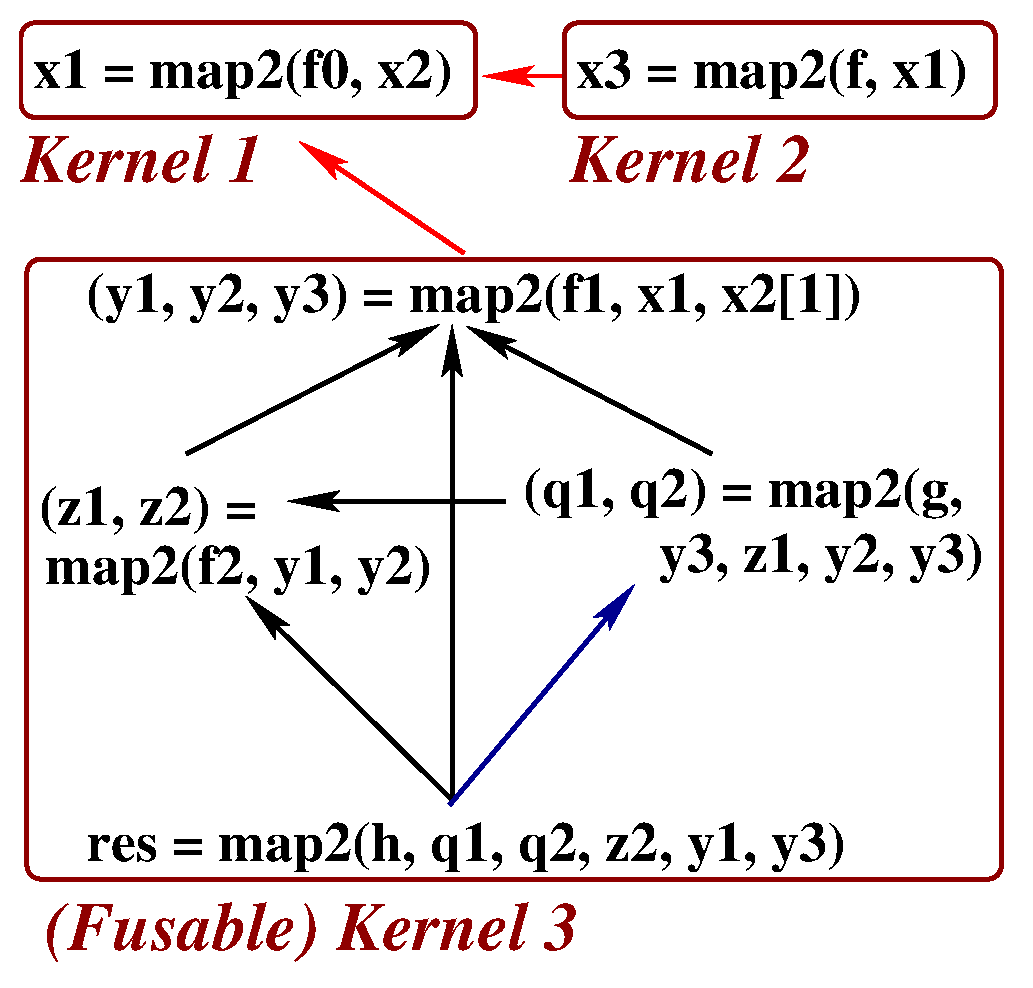
\includegraphics[height=30ex]{Figures/T1T2} \\\vspace{2ex}
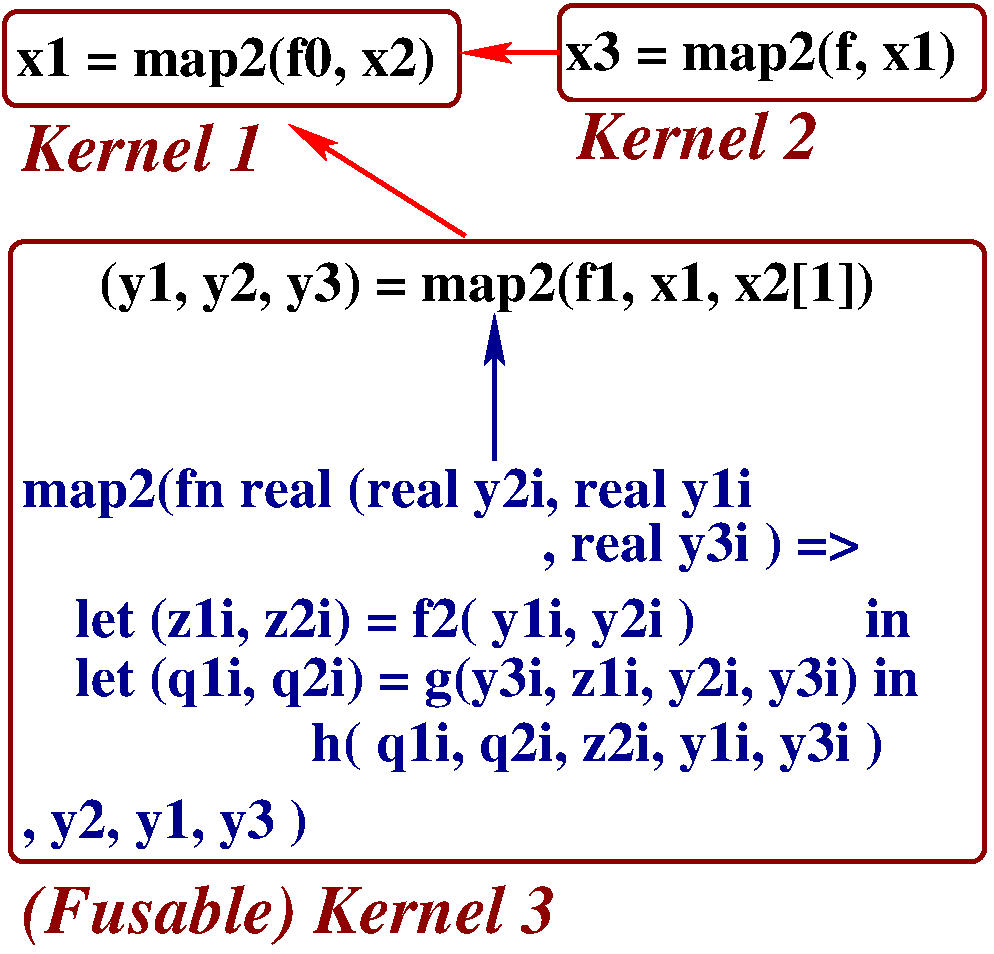
\includegraphics[height=30ex]{Figures/T1T2Fuse2}
\end{center}
\end{minipage}
\hfill
\begin{minipage}{0.46\columnwidth}
\begin{center}
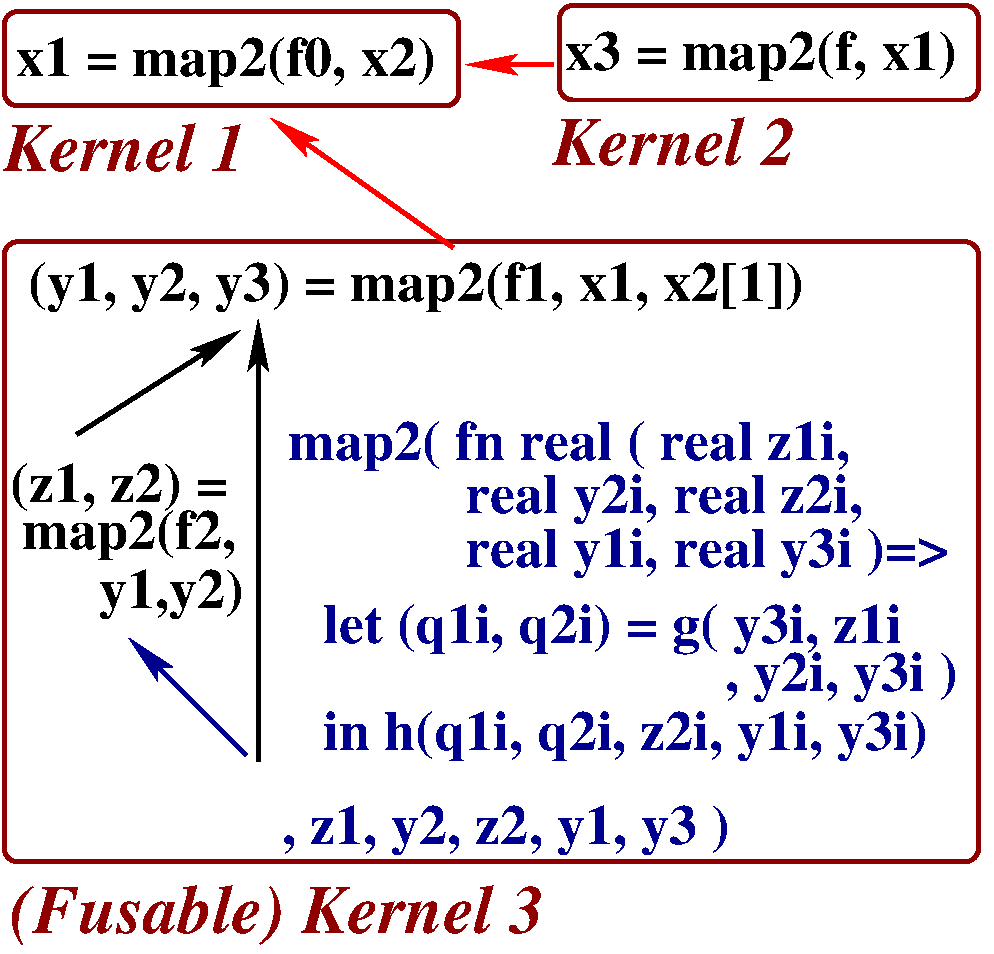
\includegraphics[height=30ex]{Figures/T1T2Fuse1} \\\vspace{2ex}
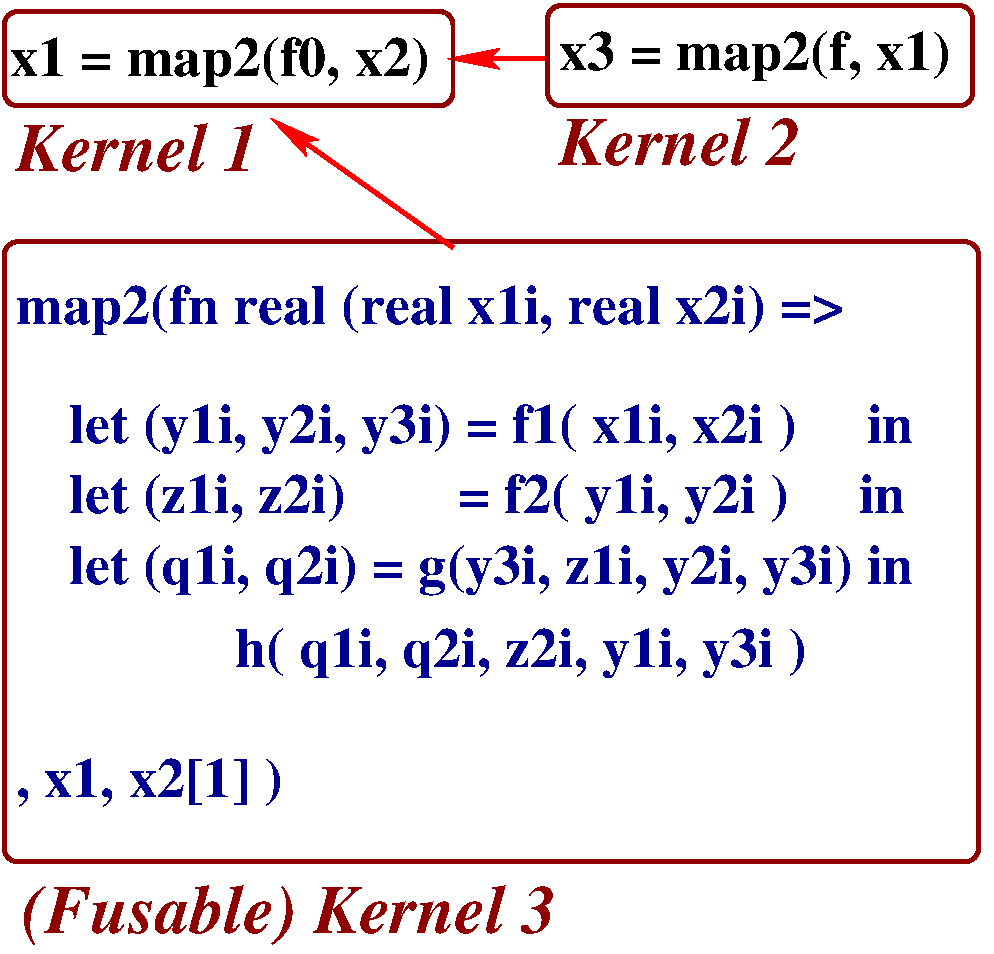
\includegraphics[height=30ex]{Figures/T1T2Fuse3}
\end{center}
\end{minipage}
%\begin{center}
%\includegraphics[height=12ex]{figures/MemCoalesce}
%\end{center}
} %\vspace{-1.5ex}
\caption{Fusion By T2 Transformation on the Dependency Graph}
\label{fig:T1T2}
\end{figure}


\begin{figure}[bt]
%\hrule ~
\vbox{
\begin{minipage}{0.48\columnwidth}
\begin{colorcode}
// \emp{Case 1:} don't fuse if it
//moves an array use across 
//its in-place update point
let \emphh{x}   = map2(f, \emp{a}) in
let \emp{a}[1]= 3.33       in
let y   = map2(g, \emp{x}) in ...

// \emp{Case 3:} not all SOAC
//combinations are fusable
let \emp{x} = filter2(c\mymath{\myindx{1}}, a) in
let \emp{y} = filter2(c\mymath{\myindx{1}}, b) in
let z = map2   (f,\emp{x,y}) in...

// \emp{Case 5:} don't fuse if \emp{x}
//used outside SOAC inputs
let \emphh{x} = map2(f, arr)  in
let y = map2(g(\emp{x}), \emphh{x}) in
\end{colorcode}
\end{minipage}
\hfill
\begin{minipage}{0.48\columnwidth}
\begin{colorcode}
// \emp{Case 2:} don't fuse from 
//outside in a loop (or \mymath{\lambda})
let \emphh{x} = map2(f, arr)   in
\emp{loop}(arr) = for i < N do
  map2(op +, arr, \emp{x})

// \emp{Case 4:} don't fuse in 2
//kernels sharing a CF path
let \emphh{x} = map2(f, arr) in
let y = map2(g, \emp{x})   in
let z = map2(h, \emp{x})   in ...

// \emp{Case 6:} x \& y used exactly
//once but still don't fuse
let (x,y) = map2(f, a)   in
let u = reduce2(op +,0,x)in
let v = reduce2(op *,1,y)...
\end{colorcode}
\end{minipage}
%\begin{center}
%\includegraphics[height=12ex]{figures/MemCoalesce}
%\end{center}
} 
%\vspace{-1ex}
\caption{Don't Fuse Cases: Illegal or Duplicates Computation}
\label{fig:dontFuse}
\end{figure}

\subsection{Fusing One SOAC}
\label{sec:FusingOnce}

\begin{figure}[bt]
%\hrule ~
\vbox{
\begin{minipage}{0.48\columnwidth}
\begin{colorcode}
import qualified Data.Map 
                 as M
import qualified Data.Set 
                 as S
data FusedKer = FusedKer \{ 
 soacStmt :: ([Ident], Exp)
--^the fused SOAC stmt,eg,
--(z,w)=map2( f(a,b), x,y )

,inp     :: S.Set Ident
--^ the input arrays used   
--in SOAC stmt,i.e.,\{x,y\}.

,inplace :: S.Set Name
--^Aliasing set of vars
--used in in-place updates
--that reach this kernel.

,fused_vars :: [Ident]
--^not null iff at least a 
--fusion has been performed
\}
\end{colorcode}
\end{minipage}
\hfill
\begin{minipage}{0.48\columnwidth}
\begin{colorcode}
data FusionRes = FusionRes\{
 outArr :: M.Map Name Name
--^maps an array to the name
--of the kernel producing it 

,inpArr :: M.Map  Name 
                (S.Set Name)
--^maps an array to the 
--names of kernels using it  

,unfused :: S.Set Name
--^Unfusable arrays. Used:
--1.otherwise than input to 
--  SOAC kernels (including
--  lambda bodies), or 
--2.as input to two kernels 
--  not located on disjoint 
--  control-flow (branches)

,kers ::M.Map Name FusedKer
--^maps kernel name to data
\}
\end{colorcode}
\end{minipage}
%\begin{center}
%\includegraphics[height=12ex]{figures/MemCoalesce}
%\end{center}
} 
%\vspace{-1ex}
\caption{Data Structures for Fusion Metadata.}
\label{fig:fusionDS}
\end{figure}


\begin{figure}[bt]
%\hrule ~
\vbox{
\begin{colorcode}
data \emphh{FusionEnv} = FusionEnv \{
    \emphh{soacsEnv} :: M.Map Name ([Name], Exp)
    --^ maps array names to their producing SOAC stmt
  , \emphh{varsEnv}  :: S.Set Name 
    --^ set of in-scope variables at current prog point
\}
newtype \emp{FusionM} a = FusionM (StateT NameSrc 
               (ReaderT FusionEnv (Either FusionErr)) a)
  deriving ( MonadState  NameSrc, MonadReader \emphh{FusionEnv},
             Monad, Applicative, Functor )

\emp{tryFuseSOAC}:: S.Set Name     ->         FusionRes -> 
             -- ^vars \mymath{\in} SOAC's lamba,   ^current result  
              ([Ident], Exp) -> \emp{FusionM} FusionRes
             -- ^SOAC stmt,      ^result after fusion
\emp{tryFuseSOAC} lam_vars res (out_ids, soac) = do   
  inp_ids <- getInpArrsSOAC soac
  --^e.g., [x,y] \mymath{\Leftarrow} map2(f, x, y)  
  inp_nms <- \emphh{expandSOACsInpArr} \$ map identName inp_ids
  --^e.g., [x,y] \mymath{\Leftarrow} map2(g, x) {\em if} let (x,y) = map2(f,a) 
  let out_nms = map identName out_idds
    
  -- \emp{Conditions for fusion:}
  --(1) \emphh{none of out_nms belongs to the unfusable set}
  let cond1=L.all (\mymath{\backslash}x->not\$ S.member x\$ unfused res) out_nms 

  --(2) \emphh{\mymath{\exists} some kernels that use some of out_ids as inputs} 
  let to_fuse_knms = getKersWithInpArrs res out_nms
  to_fuse_kers <- mapM (\mymath{\backslash}x-> case M.lookup x (kers res) of
                              Nothing -> fusionErrorM ...
                              Just ker-> return ker
                       ) to_fuse_knms
  --(3) \emphh{all kernels have to be compatible for fusion}, 
  --    e.g., map2 o filter2 not supported
  let all_compat = L.all (isCompatibleKer out_nms soac) 
                         to_fuse_kers
  --(4) \emphh{fusion cannot move a use of an input array}
  --    \emphh{past its in-place update}
  let all_used=foldl (\mymath{\backslash}y x->S.insert x y) lam_vars inp_nms
  let ok_inplace = L.all S.null \$ 
    map (S.intersection all_used . inplace) to_fuse_kers 

  let all4_ok = cond1 && not \$ null to_fuse_kers && 
                all_compat && ok_inplace
  -- \emp{Update Unfusable Set} \emphh{with the input-array names that}
  -- \emphh{appear as input arrays in kernels \mymath{\notin} to_fuse_kers},
  -- since those are input to at least 2 distinct kernels.
  let mod_kers=if is_fusable then to_fuse_knms else []
  let in2_kers=filter (inpArrInRes res mod_kers) inp_nms
  let unfused'=S.union (unfused res) (S.fromList in2_kers)
  let res' = res \{ unfused = unfused' \}

  if not all4_ok then startNewKernel res' (out_ids,soac)
             -- ^adds a fresh kernel to the result, and    
             -- updates the outArr and inpArr fields
  else do fused_kers <- mapM (fuseSOACInKer out_ids soac) 
                             to_fuse_kers
          -- ^fuses current soac with all to_fuse_kers
          updateFusionRes res' fused_kers to_fuse_knms
          -- ^updates out/inpArr \& kers fields of result
\end{colorcode}
} \vspace{-2ex}
\caption{ Conservative Fusion of a {\sc soac} }
\label{fig:FuseOnce}
\end{figure}

% map (\mymath{\backslash}k->S.intersection (inplace k) all_used) to_fuse_kers

%inpArrInResModKers
%
%addNewKer :: FusionRes -> ([Ident], Exp) -> FusionGM FusionRes
%addNewKer res (out_ids, soac) = do
%  inp_ids <- getInpArrsSOAC soac
%  inp_nms <- expandSoacInpArr \$ map identName inp_ids
%  let used_inps = filter (isInpArrInResModKers res S.empty) inp_nms
%  let unfused'  = (unfused res) `S.union` S.fromList used_inps
%
%  let new_ker = FusedKer (out_ids,soac) (S.fromList inp_ids) S.empty []    
%  nm_ker  <- freshName "ker"
%  
%  let os' = foldl (\mymath{\backslash}x arr -> M.insert arr nm_ker x) 
%                  (outArr res) (map identName out_ids)
%
%  let is' = foldl (\mymath{\backslash}x arr -> M.insertWith' S.union arr 
%                                (S.singleton nm_ker) x) 
%                  (inpArr res) inp_nms
%  return $ FusionRes os' is' unfused'  
%                     (M.insert nm_ker new_ker (kers res)) 
%

\begin{figure}[bt]
%\hrule ~
\vbox{
\begin{minipage}{0.48\columnwidth}
\begin{colorcode}
//\emp{map2 o map2 \mymath{\Rightarrow} map2}  
let (x1, x2) = map2(f, a1)
in  map2(g, x1, y)   
    \emphh{\mymath{\equiv}}
map2(fn \mymath{\beta} (\mymath{\alpha\myindx{1}} a1\mymath{\myindx{i}}, \mymath{\alpha\myindx{2}} y\mymath{\myindx{i}})
  =>let (x1\mymath{\myindx{i}}, x2\mymath{\myindx{i}}) = f(a1\mymath{\myindx{i}})
    in  g(x1\mymath{\myindx{i}}, y\mymath{\myindx{i}})
, a1, y )


//\emp{reduce2 o map2\mymath{\Rightarrow}redomap2}
let (x1, x2) = map2(f, a1)
in  reduce2(\mymath{\oplus},(e\mymath{\myindx{1}},e\mymath{\myindx{2}}),x1,y)   
    \emphh{\mymath{\equiv}}
redomap2(\mymath{\oplus}
, fn (\mymath{\beta\myindx{1}},\mymath{\beta\myindx{2}}) ( \mymath{\beta\myindx{1}} e\mymath{\myindx{1}}, \mymath{\beta\myindx{2}} e\mymath{\myindx{2}}
             , \mymath{\alpha\myindx{1}} a1\mymath{\myindx{i}},\mymath{\alpha\myindx{2}} y\mymath{\myindx{i}})
   => let (x1\mymath{\myindx{i}}, x2\mymath{\myindx{i}}) = f(a1\mymath{\myindx{i}})
      in  \mymath{\oplus}(e\mymath{\myindx{1}},e\mymath{\myindx{2}},x1\mymath{\myindx{i}},y\mymath{\myindx{i}})
, (e\mymath{\myindx{1}}, e\mymath{\myindx{2}}), a1, y )


//\emp{redomap2 o map2\mymath{\Rightarrow}redomap2}
let (x1, x2) = map2(f, a1)
in  redomap2(\mymath{\oplus}, g, e, x1, y)
    \emphh{\mymath{\equiv}}
redomap2(\mymath{\oplus}
, fn \mymath{\beta} (\mymath{\beta} e, \mymath{\alpha\myindx{1}} a1\mymath{\myindx{i}}, \mymath{\alpha\myindx{2}} y\mymath{\myindx{i}})
   => let (x1\mymath{\myindx{i}}, x2\mymath{\myindx{i}}) = f(a1\mymath{\myindx{i}})
      in  g(e, x1\mymath{\myindx{i}}, y\mymath{\myindx{i}})
, e, a1, y )


// \emp{replicate can be fused}
//\emp{without restrictions}
let x = replicate(N,a)in 
let y = map2(f, x, b) in
let z = map2(g, x, c) in 
let x[i] = ...
    \emphh{\mymath{\equiv}}
let x = replicate(N, a) in 
let y = map2( fn \mymath{\beta\myindx{1}} (\mymath{\alpha\myindx{1}} b\mymath{\myindx{i}}) 
              => f(a,b\mymath{\myindx{i}}), b)
let z = map2( fn \mymath{\beta\myindx{2}} (\mymath{\alpha\myindx{2}} c\mymath{\myindx{i}}) 
              => g(a,c\mymath{\myindx{i}}), c)
in let x[i] = ...   
\end{colorcode}
\end{minipage}
\hfill
\begin{minipage}{0.48\columnwidth}
\begin{colorcode}
//\emp{filter2 o filter2\mymath{\Rightarrow}filter2}
//\emp{{\em{}IFF} consumer's input list}
//\emp{  \mymath{\equiv} producer's output list}
let (x1,x2)=filter2(c\mymath{\myindx{1}},a1,a2)
in  filter2(c\mymath{\myindx{2}}, x1, x2)   
    \emphh{\mymath{\equiv}}
filter2(
  fn bool (\mymath{\alpha\myindx{1}} a1\mymath{\myindx{i}},\mymath{\alpha\myindx{2}} a2\mymath{\myindx{i}})=> 
      if   c\mymath{\myindx{1}}(a1\mymath{\myindx{i}}, a2\mymath{\myindx{i}}) 
      then c\mymath{\myindx{2}}(a1\mymath{\myindx{i}}, a2\mymath{\myindx{i}}) 
      else false 
, a1, a2 )

//\emp{reduce2 o filter2\mymath{\Rightarrow}redomap2}
//\emp{{\em{}IFF} consumer's input list}
//\emp{  \mymath{\equiv} producer's output list}
let x = filter2(c, a)
in  reduce2(\mymath{\oplus}, e, x)
    \emphh{\mymath{\equiv}}
reduce2(fn \mymath{\beta} (\mymath{\beta} e, \mymath{\beta} a\mymath{\myindx{i}}) =>
  if c(a\mymath{\myindx{i}}) then \mymath{\oplus}(e,a\mymath{\myindx{i}}) else e
, e, a )

//\emp{reduce2 o filter2\mymath{\Rightarrow}redomap2}
//\emp{{\em{}IFF} consumer's input set}
//\emp{  \mymath{\subseteq} producer's output set}
let (x1,x2)=filter2(c, a1, a2)
in  reduce2(\mymath{\oplus}, e, x1)
    \emphh{\mymath{\equiv}}
redomap2(\mymath{\oplus}
, fn \mymath{\beta} (\mymath{\beta} e, \mymath{\alpha\myindx{1}} a1\mymath{\myindx{i}}, \mymath{\alpha\myindx{2}} a2\mymath{\myindx{i}})
   => if c(a1\mymath{\myindx{i}}, a2\mymath{\myindx{i}})
      then \mymath{\oplus}(e, a1\mymath{\myindx{i}}) else e
, e, a1, a2 )

//\emp{redomap2 o filter2\mymath{\Rightarrow}redomap2}
//\emp{{\em{}IFF} consumer's input set}
//\emp{  \mymath{\subseteq} producer's output set}
let (x1,x2)=filter2(c, a1, a2)
in  redomap2(\mymath{\oplus}, g, e, x1)
    \emphh{\mymath{\equiv}}
redomap2(\mymath{\oplus}
, fn \mymath{\beta} (\mymath{\beta} e, \mymath{\alpha\myindx{1}} a1\mymath{\myindx{i}}, \mymath{\alpha\myindx{2}} a2\mymath{\myindx{i}})
   => if c(a1\mymath{\myindx{i}}, a2\mymath{\myindx{i}})
      then g(e, a1\mymath{\myindx{i}}) else e
, e, a1, a2 )
\end{colorcode}
\end{minipage}
%\begin{center}
%\includegraphics[height=12ex]{figures/MemCoalesce}
%\end{center}
} 
%\vspace{-1ex}
\caption{Compositional Algebra For Fusion}
\label{fig:CompatFuse}
\end{figure}



%\subsection{Fusion Structural-Analysis Algorithm}
\subsection{Building the Fused Kernels at Program Level}
\label{sec:bwdPass}

\begin{figure}[bt]
%\hrule ~
\vbox{
\begin{colorcode}
\emp{fusionGather :: FusionRes -> Exp -> FusionM FusionRes}
-----------------
-- Let Pattern --
fusionGather r (LetPat pat soac@(Map2 \mymath{\lambda} _ _ _) bdy _)=do
  r' <- \emphh{bindBothEnvs} pat soac \$ fusionGather r bdy    
  (lam_vars, r'') <- fusionGatherLam r' lam
  tryFuseSOAC lam_vars r'' (pat, soac)
-- ^similar for Reduce2, Filter2, Redomap2. 
-- ^Replicate has a specialized implem (not shown) 

fusionGather r (LetPat pat (Scan2 \mymath{\lambda} ne arr _ _) bdy _)=do
  r'        <- \emphh{bindVarsEnv} pat \$ fusionGather r bdy
  (_, r'')  <- fusionGatherLam r' \mymath{\lambda}
  foldM fusionGatherExp r'' (ne : arr)

fusionGather r (LetPat pat e body _) = do
    r' <- \emphh{bindVarsEnv} pat \$ fusionGather r body
    fusionGather r' e

fusionGather _ (Map2 \{\}) = errorIllegal ...

------------------------------------------------
-- Variable, Index, If, Loop, In-Place Update --
fusionGather r (Var idd) = do
  -- {\em If} array {\em then} add it to the unfusable set
  case identType idd of
    Array\{\} -> return \$ r \{ unfused = 
                   S.insert (identName idd) (unfused r) \}
    _       -> return \$ r

fusionGather r (Index idd indices _ _) = do 
  foldM fusionGather r ((Var idd) : indices)

fusionGather r (If e_cond e_then e_else _ _) = do
  t_r <- fusionGather mkNullRes e_then
  e_r <- fusionGather mkNullRes e_else
  c_r <- fusionGather r         e_cond
  return \$ \emp{mergeFusionRes} c_r (\emp{unionFusionRes} t_r e_r)
  -- mergeFusionRes \mymath{\equiv} semantically unions^ results, 
  --   but promotes the \mymath{\cap} of inpArr keys to unfused set

fusionGather r (LetWith id1 id0 inds elm bdy \emp{alias} _) = do 
    r'  <- \emphh{bindVarsEnv} [id1] \$ fusionGather r bdy
    -- Add the aliases set of id0 (included)
    -- to the `inplace' field of any kernel:
    let kers = M.map (\mymath{\backslash}k->k\{(inplace k) `S.union` \emp{alias}\}) 
                     (kernels r')
    foldM fusionGather (r' \{ kernels = kers \}) 
                       (elm : (Var id0) : inds)

fusionGatherLam r (AnonymFun idds body _ pos) = do
    r' <- \emphh{bindVarsEnv} idds \$ fusionGather mkNullRes body
    let inps = S.fromList \$ M.keys \$ inpArr new_res
    let unfus  = (unfused r') `S.union` inps
    -- ^make the inpArr of the \mymath{\lambda}-body result unfusable
    --  so that they cannot be fused from outside \mymath{\lambda} 
    bnds <- asks \$ varsEnv
    let unfus' = unfus `S.intersection` bnds
    -- ^filter out \mymath{\lambda}'s local vars
    return \$ (unfus', \emp{unionFusionRes} r (r'\{unfused=unfus'\}))

\end{colorcode}
} \vspace{-2ex}
\caption{ Constructing Fused Kernels at Function Level}
\label{fig:FusionGather}
\end{figure}

%fusionGather r (DoLoop arr_id ini _ ub bdy1 bdy2 _) = do
%    r'  <- \emphh{bindVarsEnv} arr_id \$ fusionGather r bdy2
%    r'' <- foldM fusionGather r' [ini,ub]
%    l_r <- \emphh{bindVarsEnv} arr_id \$ fusionGather mkNullRes bdy1
%    let inps = S.fromList \$ M.keys (inpArr l_r)
%    let l_r' = l_r\{unfused= (unfused l_r) `S.union` inps\} 
%    -- ^make the inpArr of the loop-body result unfusable
%    return \$ \emp{unionFusionRes} r'' l_r'

%tryFuseSOAC:: S.Set Name -> FusionRes -> ([Ident], Exp)-> FusionM FusionRes
%  , fusedRes   :: FusedRes


\subsection{Replacing the Fused Kernels \& Fusion Driver}
\label{sec:fwdPass}


\section{Limitations and Possible Extensions}
\label{sec:Discuss}

\begin{figure}[bt]
%\hrule ~
\vbox{
\begin{colorcode}
// \emp{Interchanging Scan With Inner Maps (ISWIM) Example}:
transpose :: [[\mymath{\alpha}]] \mymath{\rightarrow} [[\mymath{\alpha}]]
b = transpose(a) \mymath{\Rightarrow} a[i\mymath{\myindx{1}},i\mymath{\myindx{2}}] \emphh{\mymath{\equiv}} b[i\mymath{\myindx{2}},i\mymath{\myindx{1}}]

scan2( fn [real] ([real] x, [real] y) => map2(op +, x, y), 
     , \{0.0,..,0.0\}, a )   \emphh{\mymath{\equiv}}
transpose( map2 (fn [real] ([real] x)=>scan2(op +,0.0,x)
                , transpose(a) )

// \emp{Generalization for Transpose}: 
transpose :: (\mymath{{\tt Int}}, \mymath{{\tt Int}}, [\mymath{\myindx{1}}[\mymath{\myindx{..q}}\mymath{\alpha}]]) \mymath{\rightarrow} [\mymath{\myindx{1}}[\mymath{\myindx{..q}}\mymath{\alpha}]]
b=transpose(k,n,a) \mymath{\Rightarrow} a[i\mymath{\myindx{1}},..,i\mymath{\myindx{k}},i\mymath{\myindx{k+1}},..,i\mymath{\myindx{k+n}},..,i\mymath{\myindx{q}}] \emphh{\mymath{\equiv}}
                      b[i\mymath{\myindx{1}},..,i\mymath{\myindx{k+1}},..,i\mymath{\myindx{k+n}},i\mymath{\myindx{k}},..,i\mymath{\myindx{q}}] 
// \emp{Generalization for Nested Maps}:
map2\mymath{\myindu{1}}(f, a\mymath{\myindx{1}},.., a\mymath{\myindx{k}}) \emphh{\mymath{\equiv}} map2(g, a\mymath{\myindx{1}},.., a\mymath{\myindx{k}})
map2\mymath{\myindu{n}}(f, a\mymath{\myindx{1}},.., a\mymath{\myindx{k}}) \emphh{\mymath{\equiv}} 
map2(fn ([\mymath{\beta\myindx{1}}],..,[\mymath{\beta\myindx{t}}]) ([\mymath{\alpha\myindx{1}}] x\mymath{\myindx{1}},..,[\mymath{\alpha\myindx{k}}] x\mymath{\myindx{k}}) => 
        map2\mymath{\myindu{n-1}}(f, x\mymath{\myindx{1}},.., x\mymath{\myindx{k}})
    , a\mymath{\myindx{1}},.., a\mymath{\myindx{k}} )

// \emp{Fusing Across Transpose (Similar for Reshape/Flatten)}:
let x=map2\mymath{\myindu{n}}(f,a) in let y=transpose(1,n-k,x) in map2\mymath{\myindu{n}}(g,y)
        \emphh{\mymath{\equiv}}
map2\mymath{\myindu{n}}(g o f, transpose(1,n-k,a) ) 
// \emphh{i.e., the map2 produced by ISWIM may be further fused.}
\end{colorcode}
} \vspace{-2ex}
\caption{Interchange Scan With Inner Maps ({\sc iswim}) Transform.}
\label{fig:TransfEg}
\end{figure}

\begin{figure}[bt]
%\hrule ~
\vbox{
\begin{colorcode}
// \emp{Arbitrary-Nested-Level Generalization of ISWIM}:
\emp{scan2}( fn ( [\mymath{\myindx{1}}[\mymath{\myindx{..n}}\mymath{\alpha\myindx{1}}]],    .., [\mymath{\myindx{1}}[\mymath{\myindx{..n}}\mymath{\alpha\myindx{k}}]] ) 
          ( [\mymath{\myindx{1}}[\mymath{\myindx{..n}}\mymath{\alpha\myindx{1}}]] x\mymath{\myindu{1}\myindx{1}}, .., [\mymath{\myindx{1}}[\mymath{\myindx{..n}}\mymath{\alpha\myindx{k}}]] x\mymath{\myindu{1}\myindx{k}},
            [\mymath{\myindx{1}}[\mymath{\myindx{..n}}\mymath{\alpha\myindx{1}}]] x\mymath{\myindu{2}\myindx{1}}, .., [\mymath{\myindx{1}}[\mymath{\myindx{..n}}\mymath{\alpha\myindx{k}}]] x\mymath{\myindu{2}\myindx{k}} ) => 
                \emphh{map2}\mymath{\myindu{n}}(\mymath{\oplus}, x\mymath{\myindu{1}\myindx{1}},.., x\mymath{\myindu{1}\myindx{k}}, x\mymath{\myindu{2}\myindx{1}},.., x\mymath{\myindu{2}\myindx{k}}) 
     , (ne\mymath{\myindx{1}}, ..., ne\mymath{\myindx{k}}), a\mymath{\myindx{1}}, ..., a\mymath{\myindx{k}} 
     )             \emphh{\mymath{\equiv}} 
let (.., re\mymath{\myindx{t}}, ..) = (.., map\mymath{\myindu{n}}( replicate(1), ne\mymath{\myindx{t}} ), ..)
// ^replicate dim n of neutral elems so map2 sizes match
let ( y\mymath{\myindx{1}},.., y\mymath{\myindx{k}} ) =
  \emphh{map2} (fn ( [\mymath{\myindx{1}}[\mymath{\myindx{..n}}\mymath{\alpha\myindx{1}}]],    .., [\mymath{\myindx{1}}[\mymath{\myindx{..n}}\mymath{\alpha\myindx{k}}]] ) 
           ( [\mymath{\myindx{1}}[\mymath{\myindx{..n}}\mymath{\alpha\myindx{1}}]] x\mymath{\myindx{1}}, .., [\mymath{\myindx{1}}[\mymath{\myindx{..n}}\mymath{\alpha\myindx{k}}]] x\mymath{\myindx{k}} ) =>
          \emphh{map2}\mymath{\myindu{n-1}}( fn ([\mymath{\myindx{1}}[\mymath{\myindx{..n-1}}\mymath{\alpha\myindx{1}}]],  .., [\mymath{\myindx{1}}[\mymath{\myindx{..n-1}}\mymath{\alpha\myindx{k}}]] )  
                      ([\mymath{\myindx{1}}[\mymath{\myindx{..n-1}}\mymath{\alpha\myindx{1}}]] e\mymath{\myindx{1}},..,[\mymath{\myindx{1}}[\mymath{\myindx{..n-1}}\mymath{\alpha\myindx{k}}]] e\mymath{\myindx{k}}, 
                       [\mymath{\myindx{1}}[\mymath{\myindx{..n-1}}\mymath{\alpha\myindx{1}}]] x\mymath{\myindx{1}},..,[\mymath{\myindx{1}}[\mymath{\myindx{..n-1}}\mymath{\alpha\myindx{k}}]] x\mymath{\myindx{k}})
                     =>\emp{scan2}(\mymath{\oplus},(e\mymath{\myindx{1}}[0],..,e\mymath{\myindx{k}}[0]),x\mymath{\myindx{1}},..,x\mymath{\myindx{k}})
                 , re\mymath{\myindx{1}}, ..., re\mymath{\myindx{k}}, x\mymath{\myindx{1}}, .., x\mymath{\myindx{k}} )
       , transpose(1,n,a\mymath{\myindx{1}}), .., transpose(1,n,a\mymath{\myindx{k}}) )
in (transpose(n, q\mymath{\myindx{1}}-n, y\mymath{\myindx{1}}), ..., transpose(n, q\mymath{\myindx{k}}-n, y\mymath{\myindx{k}}))
// ^transpose back the result; q\mymath{\myindx{t}}-n is the dimension of \mymath{\alpha\myindx{t}}

// \emp{A Well-Known Transformation: Reduce Flattening}
y = redomap2\mymath{\myindu{n}} ( \mymath{\oplus} 
               , fn (\mymath{\alpha\myindx{1}},..,\mymath{\alpha\myindx{k}}) ( \mymath{\alpha\myindx{1}} e\mymath{\myindx{1}},..,  \mymath{\alpha\myindx{k}} e\mymath{\myindx{k}},
                                [\mymath{\alpha\myindx{1}}] x\mymath{\myindx{1}},..,[\mymath{\alpha\myindx{k}}] x\mymath{\myindx{k}} ) => 
                     reduce(\mymath{\oplus}, (e\mymath{\myindx{1}},..,e\mymath{\myindx{k}}), x\mymath{\myindx{1}},..,x\mymath{\myindx{k}})
               , (e\mymath{\myindx{1}},..,e\mymath{\myindx{k}}), a\mymath{\myindx{1}},..,a\mymath{\myindx{k}} )
        \emphh{\mymath{\equiv}}
reduce2(\mymath{\oplus}, (e\mymath{\myindx{1}},..,e\mymath{\myindx{k}}), flatten(n, a\mymath{\myindx{1}}),.., flatten(n, a\mymath{\myindx{k}}))
// ^ flatten(n,a) flattens the first n dims of array a;
// ^ redomap2\mymath{\myindu{n}} is similar to map2\mymath{\myindu{n}}
\end{colorcode}
} \vspace{-2ex}
\caption{{\sc iswim}'s Formalization \& Reduce Flattening Transform.}
\label{fig:TransfGen}
\end{figure}

%let (re\mymath{\myindx{1}},..,re\mymath{\myindx{k}} ) = map\mymath{\myindu{n}}( replicate(1), ne\mymath{\myindx{1}},.., ne\mymath{\myindx{k}} )

%  ([\mymath{\alpha\myindx{1}}] x\mymath{\myindx{1}},..,[\mymath{\alpha\myindx{k}}] x\mymath{\myindx{k}})

% Note that transpose(i+n, q-n, transpose(i, n, a)) == a

\section{Related Work}
\label{sec:RelWork}

Discuss fusion in REPA, DPH, Accelerate, Haskell, Obsidian, etc.

\section{Conclusions and Future Work}
\label{sec:Concl}



%%%%%%%%%%%%%%%%%%%%%%%%
%%% END MAIN ARTICLE %%%
%%%%%%%%%%%%%%%%%%%%%%%%

%\appendix
%\section{Appendix Title}
%
%This is the text of the appendix, if you need one.


%%%%%%%%%%%%%%%%%%%%%%%%%%%%%%%%%%%%%%%%%%%%%%%%%%%%%%%%%%%%%%%%%%%

\enlargethispage{\baselineskip}
%\vspace*{-1ex}
\acks
%\vspace*{-1ex}
This research has been partially supported by the Danish
Strategic Research Council, Program Committee for Strategic Growth
Technologies, for the research center 'HIPERFIT: Functional High
Performance Computing for Financial Information Technology'
(\url{http://hiperfit.dk}) under contract number 10-092299.


% We recommend abbrvnat bibliography style.

\bibliographystyle{abbrvnat}
\softraggedright
%\bibliography{FHPC12}

\begin{thebibliography}{49}
\providecommand{\natexlab}[1]{#1}
\providecommand{\url}[1]{\texttt{#1}}
\expandafter\ifx\csname urlstyle\endcsname\relax
  \providecommand{\doi}[1]{doi: #1}\else
  \providecommand{\doi}{doi: \begingroup \urlstyle{rm}\Url}\fi

\bibitem[Allen and Kennedy(2002)]{OptCompModernArch}
R.~Allen and K.~Kennedy.
\newblock \emph{{O}ptimizing {C}ompilers for {M}odern {A}rchitectures}.
\newblock Morgan Kaufmann, 2002.
\newblock ISBN 1-55860-286-0.

\bibitem[Amini et~al.(2011)Amini, Coelho, Irigoin, and
  Keryell]{IrigoinHostAccelOptim}
M.~Amini, F.~Coelho, F.~Irigoin, and R.~Keryell.
\newblock Static {C}ompilation {A}nalysis for {H}ost-{A}ccelerator
  {C}ommunication {O}ptimization.
\newblock In \emph{Int. Work. Lang. and Compilers for Par. Computing (LCPC)},
  2011.

\bibitem[Armstrong and Eigenmann(2008)]{GamessDif}
B.~Armstrong and R.~Eigenmann.
\newblock Application of {A}utomatic {P}arallelization to {M}odern {C}hallenges
  of {S}cientific {C}omputing {I}ndustries.
\newblock In \emph{Int. Conf. Parallel Proc. (ICPP)}, pages 279--286, 2008.

\bibitem[Augustsson et~al.(2008)Augustsson, Mansell, and
  Sittampalam]{Augustsson08Paradise}
L.~Augustsson, H.~Mansell, and G.~Sittampalam.
\newblock Paradise: {A} {T}wo-{S}tage {DSL} {E}mbedded in {Haskell}.
\newblock In \emph{Int. Conf. on Funct. Prog. (ICFP)}, pages 225--228, 2008.

\bibitem[Baskaran et~al.(2010)Baskaran, Ramanujam, and
  Sadayappan]{SadayappanCtoCUDA}
M.~M. Baskaran, J.~Ramanujam, and P.~Sadayappan.
\newblock Automatic {C}-to-{CUDA} {C}ode {G}eneration for {A}ffine {P}rograms.
\newblock In \emph{Int. Conf. on Compiler Construction (CC)}, pages 244--263,
  2010.

\bibitem[Bird(1987)]{BirdListTh}
R.~S. Bird.
\newblock An {I}ntroduction to the {T}heory of {L}ists.
\newblock In \emph{NATO Inst. on Logic of Progr. and Calculi of Discrete
  Design}, pages 5--42, 1987.

\bibitem[Black and Scholes(1973)]{black1973pricing}
F.~Black and M.~Scholes.
\newblock The {P}ricing of {O}ptions and {C}orporate {L}iabilities.
\newblock \emph{The Journal of Political Economy}, pages 637--654, 1973.

\bibitem[Blelloch(1996)]{BlellochCACM96NESL}
G.~Blelloch.
\newblock Programming {P}arallel {A}lgorithms.
\newblock \emph{Communications of the {ACM} (CACM)}, 39\penalty0 (3):\penalty0
  85--97, 1996.

\bibitem[Blume and Eigenmann(1994)]{Blume94RangeTest}
W.~Blume and R.~Eigenmann.
\newblock The {R}ange {T}est: {A} {D}ependence {T}est for {S}ymbolic,
  {N}on-{L}inear {E}xpressions.
\newblock In \emph{Procs. Int. Conf. on Supercomp}, pages 528--537, 1994.

\bibitem[Bratley and Fox(1988)]{Sobol}
P.~Bratley and B.~L. Fox.
\newblock Algorithm 659 {I}mplementing {S}obol's {Q}uasirandom {S}equence
  {G}enerator.
\newblock \emph{ACM Trans. on Math. Software (TOMS)}, 14(1):\penalty0 88--100,
  1988.

\bibitem[Chakravarty et~al.(2007)Chakravarty, Leshchinskiy, Jones, Keller, and
  Marlow]{Chak06DPH}
M.~Chakravarty, R.~Leshchinskiy, S.~P. Jones, G.~Keller, and S.~Marlow.
\newblock Data parallel {H}askell: A status report.
\newblock In \emph{Int. Work. on Declarative Aspects of Multicore Prog.
  (DAMP)}, pages 10--18, 2007.

\bibitem[Chakravarty et~al.(2011)Chakravarty, Keller, Lee, McDonell, and
  Grover]{ArrayAccelerate}
M.~M. Chakravarty, G.~Keller, S.~Lee, T.~L. McDonell, and V.~Grover.
\newblock Accelerating {H}askell {A}rray {C}odes with {M}ulticore {GPUs}.
\newblock In \emph{Int. Work. on Declarative Aspects of Multicore Prog.
  (DAMP)}, pages 3--14, 2011.

\bibitem[Cole(1993)]{ColeNearHom}
M.~Cole.
\newblock Parallel {P}rogramming, {L}ist {H}omomorphisms and the {M}aximum
  {S}egment {S}um {P}roblem.
\newblock In \emph{Procs. of Parco 93}, 1993.

\bibitem[Dang et~al.(2002)Dang, Yu, and Rauchwerger]{R-LRPD}
F.~Dang, H.~Yu, and L.~Rauchwerger.
\newblock The {R-LRPD} {T}est: {S}peculative {P}arallelization of {P}artially
  {P}arallel {L}oops.
\newblock In \emph{Int. Par. and Distr. Processing Symp. (PDPS)}, pages 20--29,
  2002.

\bibitem[Dubach et~al.(2012)Dubach, Cheng, Rabbah, Bacon, and Fink]{Lime}
C.~Dubach, P.~Cheng, R.~Rabbah, D.~F. Bacon, and S.~J. Fink.
\newblock Compiling a {H}igh-{L}evel {L}anguage for {GPU}s.
\newblock In \emph{Int. Conf. Prg. Lang. Design and Implem. (PLDI)}, pages
  1--12, 2012.

\bibitem[Feautrier(1991)]{FeautrierDataflow}
P.~Feautrier.
\newblock {D}ataflow {A}nalysis of {A}rray and {S}calar {R}eferences.
\newblock \emph{Int. Journal of Par. Prog}, 20(1):\penalty0 23--54, 1991.

\bibitem[Gibbons(1996)]{ThirdLHTh}
J.~Gibbons.
\newblock The {T}hird {H}omomorphism {T}heorem.
\newblock \emph{Journal of Functional Programming (JFP)}, 6\penalty0
  (4):\penalty0 657--665, 1996.

\bibitem[Glasserman(2004)]{glasserman2004monte}
P.~Glasserman.
\newblock \emph{Monte Carlo {M}ethods in {F}inancial {E}ngineering}.
\newblock Springer, New York, 2004.
\newblock ISBN 0387004513.

\bibitem[Gorlatch(1996{\natexlab{a}})]{Gorlatch:AntiUnif}
S.~Gorlatch.
\newblock Systematic {E}xtraction and {I}mplementation of
  {D}ivide-and-{C}onquer {P}arallelism.
\newblock In \emph{PLILP'96}, pages 274--288, 1996{\natexlab{a}}.

\bibitem[Gorlatch(1996{\natexlab{b}})]{GorlatchDistrHom}
S.~Gorlatch.
\newblock Systematic {E}fficient {P}arallelization of {S}can and {O}ther {L}ist
  {H}omomorphisms.
\newblock In \emph{Ann. European Conf. on Par. Proc. LNCS 1124}, pages
  401--408. Springer-Verlag, 1996{\natexlab{b}}.

\bibitem[Hall et~al.(2005)Hall, Amarasinghe, Murphy, Liao, and Lam]{SUIF}
M.~W. Hall, S.~P. Amarasinghe, B.~R. Murphy, S.-W. Liao, and M.~S. Lam.
\newblock Interprocedural {P}arallelization {A}nalysis in {SUIF}.
\newblock \emph{Trans. on Prog. Lang. and Sys. (TOPLAS)}, 27(4):\penalty0
  662--731, 2005.

\bibitem[Hammond and Michaelson(2000)]{HammondMichaelson00}
K.~Hammond and G.~Michaelson, editors.
\newblock \emph{{Research Directions in Parallel Functional Programming}}.
\newblock Springer, London, 2000.

\bibitem[Hu et~al.(1999)Hu, Takeichi, and Iwasaki]{HuDiffusion}
Z.~Hu, M.~Takeichi, and H.~Iwasaki.
\newblock Diffusion: {C}alculating {E}fficient {P}arallel {P}rograms.
\newblock In \emph{Int. Work. Partial Eval. and Semantics-Based Prg. Manip.
  (PEPM)}, pages 85--94, 1999.

\bibitem[Hughes(1989)]{Hughes89Why}
J.~Hughes.
\newblock Why {F}unctional {P}rogramming {M}atters.
\newblock \emph{The Computer Journal}, 32\penalty0 (2):\penalty0 98--107, 1989.

\bibitem[Hull(2009)]{hull2009options}
J.~Hull.
\newblock \emph{Options, {F}utures {A}nd {O}ther {D}erivatives}.
\newblock Prentice Hall, 2009.

\bibitem[Joshi(2010)]{joshi2010graphical}
M.~Joshi.
\newblock Graphical {A}sian {O}ptions.
\newblock \emph{Wilmott J.}, 2\penalty0 (2):\penalty0 97--107, 2010.

\bibitem[Lee et~al.(2010)Lee, Yau, Giles, Doucet, and
  Holmes]{GilesLee2010utility}
A.~Lee, C.~Yau, M.~Giles, A.~Doucet, and C.~Holmes.
\newblock On the {U}tility of {G}raphics {C}ards to {P}erform {M}assively
  {P}arallel {S}imulation of {A}dvanced {M}onte {C}arlo {M}ethods.
\newblock \emph{J. Comp. Graph. Stat}, 19\penalty0 (4):\penalty0 769--789,
  2010.

\bibitem[Lee et~al.(2009)Lee, Min, and Eigenmann]{EigenmannOpenMPtoGPU}
S.~Lee, S.-J. Min, and R.~Eigenmann.
\newblock Open{MP} to {GPGPU}: a {C}ompiler {F}ramework for {A}utomatic
  {T}ranslation and {O}ptimization.
\newblock In \emph{Int. Symp. Princ. and Practice of Par. Prog. (PPoPP)}, pages
  101--110, 2009.

\bibitem[Lin and Padua(2000)]{PaduaStackArr}
Y.~Lin and D.~Padua.
\newblock Analysis of {I}rregular {S}ingle-{I}ndexed {A}rrays and its
  {A}pplications in {C}ompiler {O}ptimizations.
\newblock In \emph{Procs. Int. Conf. on Compiler Construction}, pages 202--218,
  2000.

\bibitem[Loogen et~al.(2005)Loogen, Ortega-Mall\'{e}n, and
  {Pe\~{n}a-Mar\'{\i}}]{Eden}
R.~Loogen, Y.~Ortega-Mall\'{e}n, and R.~{Pe\~{n}a-Mar\'{\i}}.
\newblock {Parallel Functional Programming in Eden}.
\newblock \emph{J. of Funct. Prog. (JFP)}, 15\penalty0 (3):\penalty0 431--475,
  2005.

\bibitem[Lu and Mellor-Crummey.(1998)]{ExtRed}
B.~Lu and J.~Mellor-Crummey.
\newblock Compiler {O}ptimization of {I}mplicit {R}eductions for {D}istributed
  {M}emory {M}ultiprocessors.
\newblock In \emph{Int. Par. Proc. Symp. (IPPS)}, 1998.

\bibitem[Mainland and Morrisett(2010)]{Nikola}
G.~Mainland and G.~Morrisett.
\newblock {Nikola: Embedding Compiled {GPU} Functions in {H}askell}.
\newblock In \emph{Int. Symp. on Haskell}, pages 67--78, 2010.

\bibitem[Marlow et~al.(2011)Marlow, Newton, and
  Peyton~Jones]{MarlowHS11ParMonad}
S.~Marlow, R.~Newton, and S.~Peyton~Jones.
\newblock {A Monad for Deterministic Parallelism}.
\newblock In \emph{Int. Symp. on Haskell}, pages 71--82, 2011.

\bibitem[Moon and Hall(1999)]{Moon99PredArrDataFlow}
S.~Moon and M.~W. Hall.
\newblock Evaluation of {P}redicated {A}rray {D}ata-{F}low {A}nalysis for
  {A}utomatic {P}arallelization.
\newblock In \emph{Int. Symp. Princ. and Practice of Par. Prog. (PPoPP)}, pages
  84--95, 1999.

\bibitem[Morita et~al.(2007)Morita, Morihata, Matsuzaki, Hu, and
  Takeichi]{MoritaWeakInv}
K.~Morita, A.~Morihata, K.~Matsuzaki, Z.~Hu, and M.~Takeichi.
\newblock Automatic {I}nversion {G}enerates {D}ivide-and-{C}onquer {P}arallel
  {P}rograms.
\newblock In \emph{Int. Conf. Prog. Lang. Design and Impl. (PLDI)}, pages
  146--155, 2007.

\bibitem[Nord and Laure(2011)]{NordParCo11}
F.~Nord and E.~Laure.
\newblock Monte {C}arlo {O}ption {P}ricing with {G}raphics {P}rocessing
  {U}nits.
\newblock In \emph{Int. Conf. ParCo}, 2011.

\bibitem[Oancea and Rauchwerger(2012)]{CosPLDI}
C.~E. Oancea and L.~Rauchwerger.
\newblock Logical {I}nference {T}echniques for {L}oop {P}arallelization.
\newblock In \emph{Int. Conf. Prog. Lang. Design and Impl. (PLDI)}, 2012.

\bibitem[Oancea et~al.(2009)Oancea, Mycroft, and Harris]{OanceaSpLIP}
C.~E. Oancea, A.~Mycroft, and T.~Harris.
\newblock A {L}ightweight, {I}n-{P}lace {M}odel for {S}oftware {T}hread-{L}evel
  {S}peculation.
\newblock In \emph{Int. Symp. on Par. Alg. Arch. (SPAA)}, pages 223--232, 2009.

\bibitem[Paek et~al.(2002)Paek, Hoeflinger, and Padua]{LMAD}
Y.~Paek, J.~Hoeflinger, and D.~Padua.
\newblock Efficient and {P}recise {A}rray {A}ccess {A}nalysis.
\newblock \emph{Trans. on Prog. Lang. and Sys. (TOPLAS)}, 24(1):\penalty0
  65--109, 2002.

\bibitem[{Peyton Jones} et~al.(2000){Peyton Jones}, Eber, and Seward]{SPJ00}
S.~{Peyton Jones}, J.-M. Eber, and J.~Seward.
\newblock Composing {C}ontracts: an {A}dventure in {F}inancial {E}ngineering
  (functional pearl).
\newblock In \emph{Int. Conf. on Funct. Prog. (ICFP)}, pages 280--292, 2000.

\bibitem[Pouchet and et~al.(2012)]{PolyhedralOpt}
L.~Pouchet and et~al.
\newblock Loop {T}ransformations: {C}onvexity, {P}runing and {O}ptimization.
\newblock In \emph{Int. Conf. Princ. of Prog. Lang. (POPL)}, 2012.

\bibitem[Pugh and Wonnacott(1998)]{Pugh98NonlinPresb}
W.~Pugh and D.~Wonnacott.
\newblock Constraint-{B}ased {A}rray {D}ependence {A}nalysis.
\newblock \emph{Trans. on Prog. Lang. and Sys.}, 20(3):\penalty0 635--678,
  1998.

\bibitem[Rus et~al.(2003)Rus, Hoeflinger, and Rauchwerger]{HybAn}
S.~Rus, J.~Hoeflinger, and L.~Rauchwerger.
\newblock Hybrid {A}nalysis: {S}tatic \& {D}ynamic {M}emory {R}eference
  {A}nalysis.
\newblock \emph{Int. Journal of Par. Prog}, 31(3):\penalty0 251--283, 2003.

\bibitem[Ryoo et~al.(2008)Ryoo, Rodrigues, Baghsorkhi, Stone, Kirk, and
  Hwu]{PrinciplesMemGPU}
S.~Ryoo, C.~I. Rodrigues, S.~S. Baghsorkhi, S.~S. Stone, D.~B. Kirk, and
  W.-m.~W. Hwu.
\newblock Optimization {P}rinciples and {A}pplication {P}erformance
  {E}valuation of a {M}ultithreaded {GPU} {U}sing {CUDA}.
\newblock In \emph{Int. Symp. Princ. and Practice of Par. Prog. (PPoPP)}, pages
  73--82, 2008.

\bibitem[Strout(2003)]{StroutPhD}
M.~M. Strout.
\newblock \emph{Performance transformations for irregular applications}.
\newblock PhD thesis, 2003.
\newblock AAI3094622.

\bibitem[Trinder et~al.(1996)Trinder, Hammond, {Mattson Jr.}, Partridge, and
  {Peyton Jones}]{GpH}
P.~Trinder, K.~Hammond, J.~{Mattson Jr.}, A.~Partridge, and S.~{Peyton Jones}.
\newblock {GUM: a Portable Parallel Implementation of Haskell}.
\newblock In \emph{Int. Conf. Prg. Lang. Design and Implem. (PLDI)}, pages
  78--88, 1996.

\bibitem[Ueng et~al.(2008)Ueng, Lathara, Baghsorkhi, and Hwu]{CudaLite}
S.-Z. Ueng, M.~Lathara, S.~S. Baghsorkhi, and W.-M.~W. Hwu.
\newblock {CUDA}-{L}ite: {R}educing {GPU} {P}rogramming {C}omplexity.
\newblock In \emph{Int. Work. Lang. and Compilers for Par. Computing (LCPC)},
  pages 1--15, 2008.

\bibitem[Wichura(1988)]{wichura1988algorithm}
M.~Wichura.
\newblock Algorithm {AS} 241: {T}he percentage points of the {N}ormal
  distribution.
\newblock \emph{Journal of the Royal Statistical Society. Series C (Applied
  Statistics)}, 37\penalty0 (3):\penalty0 477--484, 1988.

\bibitem[Yang et~al.(2010)Yang, Xiang, Kong, and Zhou]{YangMemOptim}
Y.~Yang, P.~Xiang, J.~Kong, and H.~Zhou.
\newblock A {GPGPU} {C}ompiler for {M}emory {O}ptimization and {P}arallelism
  {M}anagement.
\newblock In \emph{Int. Conf. Prog. Lang. Design and Implem. (PLDI)}, pages
  86--97, 2010.

\end{thebibliography}

\end{document}
